\documentclass[../thesis.tex]{subfiles}
 
\begin{document}
 
 
\section{Sample-Based Planning}
\label{sec:sample_based_planning}
 
Sample-based planners search for the feasible paths through the configuration space in a probabilistic fashion.
Similar to graph-based approaches, the validity of configuration space need not be explicitly formulated; instead, we only need a function that determines whether a specific configuration is valid.
The probabilistic property makes sample-based planners suitable to tackle high dimensional configuration space planning problems, yet with the trade-off on the sub-optimality of the solution.
The Rapidly-exploring Random Tree (RRT) is a sampling-based planner which build trees of valid trajectories (edges) between points in configuration space (nodes).
As shown in Algorithm \ref{alg:RRT} \cite{lavalle1998rapidly}, to grow these graphs, a new point in configuration space is sampled, and the closest point on the existing tree is extended towards this sampled point.
 
\begin{algorithm}
  \caption{RRT} \label{alg:RRT}
  \begin{algorithmic}[1]
  \State $T \leftarrow$ InitTree( $x_{start}$ )
  \While {GoalNotReached($T, X_{goal}$)}
        \State $x_{sample} \in X \leftarrow$ Sample()
        \State $x_{nearest} \leftarrow $ Nearest($T, x_{sample}$)
        \State $x_{new} \leftarrow $ Extend($x_{nearest}, x_{sample}$)
        \State T $\leftarrow $UpdateTree($(x_{nearest},x_{new}), T)$)
  \EndWhile
  \end{algorithmic}
\end{algorithm}
 
The Extend function constructs a linearly trajectory in the configuration space from $x_{nearest}$ towards $x_{sample}$.
The extension terminates at $x_{new}$ either when $x_{sample}$ is reached, or when the trajectory enters an invalid region, which can be specified by the validity function mentioned in the previous paragraph, or a hyper-parameter \textit{step size}.
However, the standard RRT planner does not guarantee optimality of the solution.
 
\citet{karaman2011sampling} proposes an extended version of RRT that follows an asymptotic convergence to the optimal solution.
As shown in Algorithm \ref{alg:RRT_star}, the new algorithm, named RRT*, preserves the original structure yet embeds the following two additional procedures.
 
\begin{enumerate}
 
      \item Instead of extending the tree from $x_{nearest}$ towards $x_{new}$, we search on a subset $X_{near}$ centered at $x_{nearest}$ to find an alternative candidate. The new node $x_{min}$ should be collision free and follows the constraint: $cost(x_{start},x_{min}) + cost(x_{min}, x_{new}) < cost(x_{start},x_{nearest}) + cost(x_{nearest}, x_{new})$.
      
      \item Replace the original edges from $x_{min}$ to $x_{nearest}$ with $E(x_{min}, x{new})$ and $E(x_{new}, x_{nearest})$ if the resulting trajectory has lesser cost.
 
\end{enumerate}
 
\begin{algorithm}
  \caption{New Extend and Update Function in RRT*} \label{alg:RRT_star}
  \begin{algorithmic}[1]
  \State $x_{new} \leftarrow $ Extend($x_{nearest}, x_{sample}$)
  \State $X_{min} \leftarrow $ LocalSearch($T, x_{nearest}$)
  \State $x_{min} \leftarrow x_{nearest}$
  \ForEach {$x \in X_{min} $}
    \State $oldCost \leftarrow cost(x_{start},x_{nearest}) + cost(x_{nearest}, x_{new})$
    \State $newCost \leftarrow cost(x_{start},x) + cost(x, x_{new})$
    \If {$ newCost < oldCost $}
    \State $x_{min} \leftarrow x$
    \EndIf
  \EndFor
  \State T $\leftarrow $ UpdateTree($(x_{min},x_{new}), T)$)
  \ForEach {$x \in X_{min} $}
    \State $oldCost \leftarrow cost(x, x_{nearest})$
    \State $newCost \leftarrow cost(x_{new}, x_{nearest})$
      \If {$ newCost < oldCost $}
          \State $E \leftarrow E \setminus (x, x_{nearest})$
          \State $E \leftarrow E \cup (x_{new}, x_{nearest})$
    \EndIf
  \EndFor
  \end{algorithmic}
\end{algorithm}
 

 
 
\section{Deep Reinforcement Learning (DRL)}
% \label{sec:mdrl-background}
% \subsection{}
 
%% general introduction of RL notation and several useful functions (Q, V, A, mu, ...) %%%
 
We consider a standard Reinforcement Learning (RL) setup, where an agent operates in an environment ${E}$. At each discrete time step $t$, the agent observes a state $s_t \in \mathcal{S}$, picks an action $a_t \in \mathcal{A}$, and receives a scalar reward $r(s_t, a_t) \in \mathbb{R}$ from the environment. The return $R_t = \sum^T_{i=t} \gamma^{(i-t)}r(s_i,a_i)$ is defined as total discounted future reward at time step $t$, with $\gamma$ being a discount factor $\in [0,1]$. The objective of the agent is to learn a policy that eventually maximizes the expected return, as shown below:
 
\begin{align}
\centering
J = \mathbb{E}_{s_i, r_i \sim E~, a_i \sim \pi}[R_1] \label{equ:obj-func}
\end{align}
 
The learned policy, $\pi$, can be formulated as either stochastic $\pi(a|s) = \mathbb{P}(a|s)$, or deterministic $a = \mu(s)$. The value function $V^{\pi}$ and action-value function $Q^{\pi}$ describe the expected return for each state and state-action pair upon following a policy $\pi$.
 
\begin{align}
V^\pi(s_t) &= \mathbb{E}_{r_{i \geq t}, s_{i > t} \sim E, a_{i \geq t} \sim \pi} [R_t | a_t, s_t] \\
Q^\pi(s_t, a_t) &= \mathbb{E}_{r_{i \geq t}, s_{i > t} \sim E} [r(s_t, a_t) \nonumber \\
&\qquad + \gamma \mathbb{E}_{a_{i > t} \sim \pi} [Q^\pi(s_{t+1}, a_{t+1})]]
\end{align}
 
Finally, an advantage function $A^{\pi}(s_t,a_t)$ is defined as the additional return or advantage that the agent will have for executing some action $a_t$ at state $s_t$ and it is given by $A^{\pi}(s_t,a_t) = Q^\pi(s_t, a_t) - V^\pi(s_t)$.
 
%% Deep architecture on RL -> DRL! %%%
 
In high-dimensional state/action spaces, these functions are usually approximated by a suitable parametrization. 
Accordingly, we define $\theta^Q$, $\theta^V$, $\theta^A$, $\theta^\pi$, and $\theta^\mu$ as the parameters for approximating $Q$, $V$, $A$, $\pi$, and $\mu$ functions, respectively. 
It was believed that using nonlinear function approximators for both $Q$ and $V$ functions would lead to unstable learning in practice. 
Recently, \citet{mnih2013playing} applies two novel modifications, namely \textit{replay buffer} and \textit{target network}, to stabilize the learning with deep nets. 
Later, several variants are introduced and extend deep architectures to learning tasks with continuous actions \cite{DBLP:journals/corr/LillicrapHPHETS15,A3C,CDQN,TRPO}.
 
To exhaustively analyze the effect of multi-sensor input on our proposed method, we pick two algorithms, namely Normalized Advantage Function (NAF) \cite{CDQN} and Deep Deterministic Policy Gradient (DDPG) \cite{DBLP:journals/corr/LillicrapHPHETS15}, and augment them to accept multimodal inputs. 
It is worth noting that the two algorithms are very different, with DDPG being an off-policy actor-critic method and NAF an off-policy value-based one. 
By augmenting these two algorithms, we highlight that any DRL algorithm, modified appropriately, can benefit from using multiple inputs. 
% Before introducing the multimodal architecture, we briefly summarize the two algorithms below.

 
\subsection{Continuous Action Space Algorithms}
 
\subsubsection{Normalized Advantage Function (NAF)}
\label{sec:CDQN}
 
%%% Q-learning %%%
Q-learning \cite{sutton1999policy} is an off-policy model-free algorithm, where agent learns an approximated $Q$ function, and follows a greedy policy $\mu(s)=\arg\max_aQ(s,a)$ at each step. The objective function (\ref{equ:obj-func}) can be reached by minimizing the square loss Bellman error
 
\begin{align}
\centering
L = \frac{1}{N} \sum_i^N (y_i-Q(s_i,a_i|\theta^Q))^2
\end{align}
 
where target $y_i$ is defined as $r(s_i,a_i) + \gamma Q(s_{i+1},\mu(s_{i+1}))$.
 
%%% DQN and C-DQN %%%
 
Deep Q-Network (DQN) parametrizes $Q$ function with deep neural network \cite{mnih2013playing}, and has been shown to emulate human performance \cite{mnih2015human} in many Atari games using just image pixels as input. However, in these games, action choices are limited and discrete. Recently, \citet{CDQN} proposes a continuous variant of DQN by a clever network construction. The $Q$ network, which they call Normalized Advantage Function (NAF), parameterizes the advantage function quadratically over the action space and is weighted by nonlinear features of states.

\begin{align}
\centering
Q(s,a|\theta^Q) &= A(s,a | \theta^\mu, \theta^L) + V(s|\theta^V) \\
A(s,a | \theta^\mu, \theta^L) &= -\frac{1}{2}(a-\mu(s|\theta^\mu))^T P(s|\theta^L)\nonumber \\
&\qquad \qquad \qquad(a-\mu(s|\theta^\mu)) \label{equ:NAF} \\
P(s|\theta^L) &= L(s|\theta^L)^TL(s|\theta^L) \label{equ:P}
\end{align}
During run-time, the greedy policy can be performed by simply taking the output of sub-network $a = \mu(s|\theta^\mu)$. The data flow at forward prediction and back-propagation steps are shown in Fig. \ref{fig:CDQN-DDPG} (a) and (b), respectively.
 
\begin{figure}[t]
  \begin{center}
  \centerline{
\includegraphics[width=0.8\columnwidth,trim= 80 900 110 70, clip=true]{./MultimodalDRL/fig/naf_ddpg}}
  \caption{Schematic illustration of (a) forward and (b) back-propagation for NAF, and (c) forward and (d) back-propagation for DDPG. Green modules are functions approximated with deep nets.}
  \label{fig:CDQN-DDPG}
  \end{center}
  \vskip -0.5in
\end{figure}
 
\subsubsection{Deep Deterministic Policy Gradient (DDPG)}
%%% Actor-Critic and DPG %%%
An alternative approach to continuous RL tasks is the actor-critic framework, which maintains an explicit policy function, often called \textit{actor}, and an action-value function called \textit{critic}.
In \cite{dpg}, a novel \emph{deterministic} policy gradient (DPG) approach is proposed. \citet{dpg} shows that the objective function can be achieved using the policy gradient calculated from the gradient of the action-value function.
% has a model-free form and follows the gradient of the action-value function.
 
\begin{equation}
\nabla_{\theta^\mu} J = \mathbb{E}[\nabla_a Q(s,a|\theta^Q) \nabla_a \mu(s)]
\label{dpg}
\end{equation}

% \citet{dpg} proves that using the policy gradient calculated in (\ref{dpg}) to update model parameters leads to the maximum expected reward.
 
%%% DDPG %%%
Building on this result, \citet{DBLP:journals/corr/LillicrapHPHETS15} proposes an extension of DPG with deep architecture to generalize their prior success with discrete action space \cite{mnih2015human} onto continuous space. 
% Using the DPG, an off-policy algorithm is developed to estimate the $Q$ function using a differentiable function approximator. 
Similar techniques as in \cite{mnih2015human} are utilized for stable learning. 
To explore the full state and action space, an exploration policy is constructed by adding Ornstein-Uhlenbeck noise process \cite{uhlenbeck1930theory}. 
% In short, actions are chosen stochastically but a deterministic policy gradient is learned. 
The data flow for prediction and back-propagation steps are shown in Fig. \ref{fig:CDQN-DDPG} (c) and (d), respectively.
 
 
\section{Stochastic regularization}
 
Stochastic regularization is an active area of research in deep learning made popular by the success of, \textit{Dropout} \cite{dropout}. Following this landmark paper, numerous extensions are proposed to further generalize this idea such as \textit{Blockout} \cite{blockout}, \textit{DropConnect} \cite{dropconnect}, \textit{Zoneout} \cite{zoneout}, etc. 
In the similar vein, two interesting techniques have been proposed for specialized regularization in the multimodal setting namely ModDrop \cite{moddrop} and ModOut \cite{modout}.
Given a much wider set of sensors to choose from, ModOut attempts to identify which sensors are needed to fully observe the system behavior, which is out of the scope of this work. 
Here, we assume that all the sensors are critical and we only focus on improving the state information based on inputs from multiple observers.
ModDrop is much closer in spirit to the proposed \emph{Sensor Dropout (SD)}. 
However, unlike ModDrop, pre-training with individual sensor inputs using separate loss functions is not required. 
A network can be directly constructed in an end-to-end fashion and \emph{Sensor Dropout} can be directly applied to the sensor fusion layer just like Dropout. 
Its appeal lies in its simplicity during implementation and is designed to be applicable even to the DRL setting. 
As far as we know, this is the first attempt at applying stochastic regularization in a DRL setting with the spirit of sensor fusion.
 
 
%%%%%%%%%%%%%%%%%%%%%%%%%%%%%%%%%%%%%%%%%%%%%%%%%%%%%%%%%%%%%%%%%%%%%%%%%%%%%%%%%%%%%%%%%%%%%%%%%%%%%%%%%%%%%%%%%%%%%%
 
\section{Deep Inverse Reinforcement Learning (DIRL)}
\label{sec:dirl_intro}
 
%%% Formulation of IRL %%%
 
\begin{figure}[b]
      % \vskip -0.5in
      \begin{center}
       \centerline{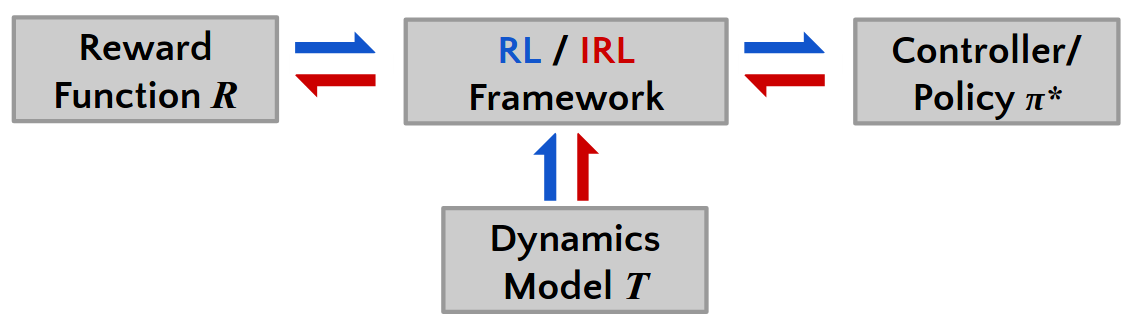
\includegraphics[width=0.5\columnwidth]{./DIRL/fig/irl_rl_pipeline.png}}
            \caption{The block diagram of reinforcement learning and inverse reinforcement learning.}
            \label{fig:irl_rl}
      \end{center}
      % \vskip -0.5in
\end{figure}
 
As shown in Fig. \ref{fig:irl_rl}, in the standard reinforcement learning, we are interested in learning the optimal policy that maximizes the total expected rewards collected from the environment.
However, for some of the interesting problems in robotics fields, designing reward functions can be non-trivial and often requires lots of handy tunings.
On the other hand, the consequences of the policy are usually relatively easy to observe.
These problems fall in the category of \textit{inverse} reinforcement learning (IRL) \cite{ng2000algorithms} (also imitation learning, learning from demonstration).
 
 
%%% IRL as a Maximum Margin Planning %%%
 
Given a set of expert demonstrations $D=\left\{ \xi_i \right\}_{i=1}^{N}$, where each trajectory $\xi_i$ consists of a sequence of state-action pair $\xi_i = \left\{ (s_j, a_j) \right\}_{j=1}^{K}$, the goal of IRL is to infer the underlying reward function that leads to the policy $\pi$.
We parametrize the reward function $r$ with $\theta$. \citet{abbeel2004apprenticeship} proposes a strategy of matching feature expectations between the demonstration policy and the learner's behavior. 
\citet{ratliff2006maximum} proposes a clever framework named \textit{Maximum Margin Planning} (MMP), where learning to plan by mimicking the expert behavior is cast as a structured prediction problem. Under the structured margin criteria, the objective can be formulated in the following form:
 
% Under the standard definition of Markov Decision Process (MDP).
\begin{align}
L(\theta) = \frac{1}{N} \sum^{N}_{i=1} \beta_i ( \max_{\mu \in \mathbb{G}_i}(\theta^T F_i + l_i^T)\mu - \theta^TF_i\mu_i )^q +  \frac{\lambda}{2} \| \theta \|^2 \label{equ:mmp_obj}
\end{align}

Here, $\mu_i$, $F_i$, and $l_i$ represent the state visited frequencies (SVF), feature matrix, and margin loss vector of the $i^{th}$ trajectory, respectively.
Note that Eq. \ref{equ:mmp_obj} assumes the linearity constraint on the reward function.
The parameter $\theta$ is optimized in a way that minimizes the $q$-norm mean losses between the optimal trajectory under the loss-augmented reward structure and the demonstration trajectories.
The loss vector alleviates the ill-posed problem in the IRL \cite{abbeel2004apprenticeship}, where a trivial solution like all-zeroed weights guarantees all policies to be optimal.
The intuition behind MMP implies the resulting solution should look significantly better than the alternative policies.
 
%%% ME-IRL %%%
However, both approaches fail to capture the ambiguity of the observed policies.
It is worth mentioning that for complex problems such as off-road navigation and racing planning, the assumption on the optimality of the demonstrations is indeed strong. 
In fact, the optimal policy is usually unknown, and the behavior may differ from each expert player.
Specifically, when the demonstrations are imperfect, or the planning algorithms capture only part of the relevant feature space, the resulting reward function from the previous approaches cannot perfectly describe the observed trajectories.
In this light, \citet{ziebart2008maximum} reformulates the problem under the principle of maximum entropy.
The resulting algorithm, known as maximum entropy IRL (ME-IRL), models the demonstrations with a stochastic policy by assuming the probability of executing of each trajectory being exponentially proportional to its total accumulated rewards.
The gradient of the objective function under linear reward function is simply the difference between the expected empirical feature counts and the learner's expected feature counts.
 
 
%%% ME-DIRL %%%
 
\begin{figure}[t]
      \begin{center}
       \centerline{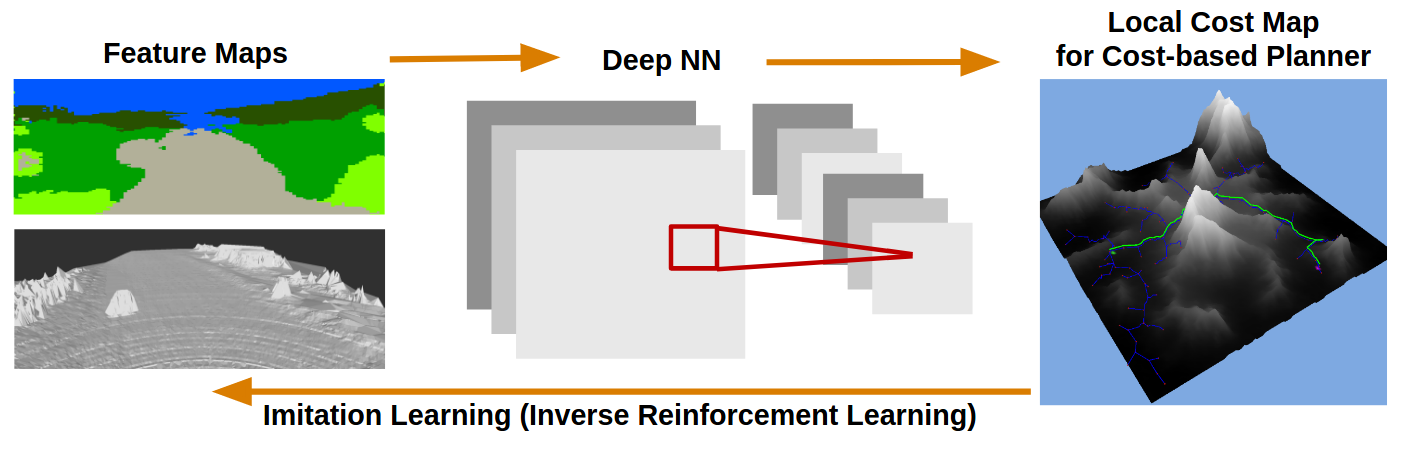
\includegraphics[width=0.9\columnwidth]{./DIRL/fig/dirl_pipeline.png}}
            \caption{Schematic illustration of deep inverse reinforcement learning.}
            \label{fig:dirl_diagram}
      \end{center}
      \vskip -0.5in
\end{figure}
 
Recently, \citet{wulfmeier2015maximum} shows that the gradient calculated in ME-IRL can be naturally extended to the back-propagation in the standard deep supervised learning.
By re-framing the problem with standard Bayesian inference as a MAP estimation problem, the objective function is simply:
 
\begin{align}
L(\theta) = \log P(D,\theta|r) = \log P(D|r) + \log P(\theta) \label{equ:dirl_obj}
\end{align}
 
The negative log-likelihood contains two terms: the data term $L_{D}$ and a standard weight decay term $L_{\theta}$ as the regularization.
The gradient of the first term is simply:
 
\begin{align}
\frac{\partial L_D}{\partial \theta} &= \frac{\partial L_D}{\partial r} \frac{\partial r}{\partial \theta} \\
&= (\mu_D - \mathbb{E}[\mu]) \cdot \frac{\partial r}{\partial \theta} \label{equ:dirl_grad}
\end{align}
 
Note the gradient degenerates to ME-IRL if the reward function is linear on feature space.
If the reward function $r$ is approximated by a deep network, the latter term $\partial r / \partial \theta$ can be calculated efficiently using back-propagation, and the objective function can be optimized with gradient-based approaches.
This framework, called deep maximum entropy deep inverse reinforcement learning (ME-DIRL or simply DIRL) has been successfully applied to urban autonomous navigation in \cite{wulfmeier2016watch}.
The schematic illustration of the DIRL is summarized in Fig. \ref{fig:dirl_diagram}.
 
%%% Other Non-linear IRL %%%
% An alternative for non-linear IRL is to use Gaussian process \cite{levine2011nonlinear}.
 
%%% Connections to MMP and MEIRL %%%
% However, the two formulations can be generalized in a unification.
 
 
\end{document}
